\documentclass[11pt]{article}
\usepackage[margin=1in]{geometry}
\usepackage[dvipsnames]{xcolor}
\usepackage{amsmath,amssymb,amsfonts,amsthm}
\usepackage{mathtools}
\usepackage{bm}
\usepackage{booktabs}
\usepackage{hyperref}
\usepackage{url}
\usepackage{graphicx}
\usepackage{authblk}

\hypersetup{colorlinks=true,linkcolor=blue,citecolor=blue,urlcolor=blue}

\newcommand{\R}{\mathbb{R}}
\newcommand{\cO}{\mathcal{O}}

\newtheorem{theorem}{Theorem}
\newtheorem{proposition}[theorem]{Proposition}

\title{SANATAN\textsuperscript{*}: Root-Parity Gated Angular Attention \\ with an Exact Constant-State Recurrent Form}

\author[ ]{Bhargav Patel}
\affil[ ]{Independent Researcher, Greater Sudbury, Ontario, Canada}
\affil[ ]{\texttt{b.patel.physics@gmail.com} \quad ORCID: 0009-0004-5429-2771}
\date{}

\begin{document}
\maketitle
\renewcommand{\thefootnote}{*}
\footnotetext{From Sanskrit \emph{san\={a}tana}, meaning ``eternal'' or ``timeless,'' reflecting the constant-size inference state. This manuscript is a corrected and extended revision of a NeurIPS 2026 submission; Appendix~\ref{app:changelog} lists every substantive change, including retracted results.}
\renewcommand{\thefootnote}{\arabic{footnote}}

\begin{abstract}
Standard self-attention requires a key--value cache that grows linearly with sequence length, making long-context decoding progressively more expensive. This paper introduces SANATAN, a linear attention mechanism built on \emph{root-parity gating}: over $2 \times 2$ real matrices, $i^2 = -1$ has two canonical orthogonal solutions, and each feature dimension of a token softly selects one of them, yielding a $d$-bit binary label that gates per-dimension interaction between queries and keys inside an angular kernel. In the linear ($p{=}1$) case the mechanism admits an exact constant-size recurrent state. We implement and verify this recurrence: on a trained 184M-parameter model, parallel and recurrent computation agree to within $10^{-4}$ nats in loss, and the constant-state model matches its full parallel parent in quality (3.951 versus 3.966 held-out loss) while decoding with a fixed 14.4\,MB state and 0.153\,ms per token, a $3.2\times$ to $48\times$ latency advantage over softmax KV-cache decoding at context lengths from 1K to 32K. We further measure that applying the recurrence to models trained with polynomial sharpening ($p{>}1$) degrades loss by roughly 5 nats, establishing that the constant-state claim holds only for $p{=}1$-trained models, and we show that a two-stage recipe (sharpened pretraining followed by brief $p{=}1$ adaptation) recovers constant-state quality that single-stage $p{=}1$ training does not reach at the same budget. On a common seeded held-out protocol, SANATAN outperforms the evaluated pre-2022 constant-memory attention baselines under a shared recipe (best: Linear Transformer at 4.524), while a matched-recipe Gated Linear Attention baseline reaches 3.348 and trains $5.5\times$ faster, so SANATAN is not yet competitive with modern gated linear attention; the contribution of this paper is the root-parity mechanism itself, its measured ablation value ($+0.53$ nats over the ungated angular kernel), its verified exact constant-state form, and a corrected evaluation methodology, including the retraction of one result from the earlier version of this work.
\end{abstract}

\section{Introduction}
\label{sec:intro}

Self-attention~\cite{vaswani2017attention} carries an inference cost that scales with sequence length: at each new position, a key--value entry is appended to a cache that grows without bound. Existing efficient-attention work either preserves all tokens and accelerates softmax over them~\cite{dao2022flashattention, wang2020linformer}, or compresses tokens into a constant-size state. Classical linear attention~\cite{katharopoulos2020transformers, choromanski2021rethinking} compresses without decay but folds all tokens into an unstructured representation; modern recurrent architectures such as RetNet, RWKV, Mamba, and gated linear attention~\cite{sun2023retnet, peng2023rwkv, gu2023mamba, yang2024gla} compress with learned decay or data-dependent gating of the \emph{state}. This paper explores a different axis: gating the pairwise \emph{interaction} itself, per dimension, by a binary label derived from algebra rather than learned from scratch.

Over $2 \times 2$ real matrices, the equation $i^2 = -1$---which has the two scalar complex solutions $+i$ and $-i$---admits two canonical orthogonal matrix solutions, $i_+$ and $i_-$, the real-matrix representations of these two orientations~\cite{patel2025quantuminspired}. Treating the choice of root as a binary label, mapping each feature dimension to an angle on a circle, and chaining $d$ circles yields a $d$-bit code over the torus $\mathbb{T}^d$: queries and keys interact on a dimension only when their root labels agree there. The $2^d$ count describes the size of this \emph{label space}; as we make precise in Section~\ref{sec:analysis}, the mechanism provides near-binary per-dimension gating rather than isolation between full label patterns, and we quantify the realized gating behavior of the trained model directly.

The mechanism is realized by a six-channel feature map whose pairwise score factorizes exactly into a parity gate and an angular similarity, position is encoded by a bounded learned phase rotation, and polynomial sharpening replaces the softmax exponential because it preserves the gate's zero. In the linear case the whole model admits an exact constant-state recurrence, which we implement, verify numerically against the parallel computation, and benchmark against softmax KV-cache decoding.

\paragraph{Contributions.}
\emph{(i)} Root parity as a gated angular attention mechanism: an algebraically derived, per-dimension binary gate inside a linear-attention kernel, with exact (six-path) and relaxed (four-path) realizations (Sections~\ref{sec:algebra}--\ref{sec:method}).
\emph{(ii)} A verified exact constant-state inference form: the $p{=}1$ recurrence agrees with parallel computation to within $10^{-4}$ nats on the trained model, and a two-stage training recipe (sharpened pretraining, then brief $p{=}1$ adaptation) preserves quality under the exact constant state (3.951 versus 3.966 for the parallel parent). We also measure that recurrent deployment of $p{>}1$-trained models is not viable ($\approx{+}5$ nats) (Sections~\ref{sec:recurrent}, \ref{sec:experiments}).
\emph{(iii)} A measured memory/latency breakeven against correctly accounted softmax KV-cache decoding: constant 14.4\,MB state versus a cache that crosses over at roughly $n \approx 195$ tokens, and a $3.2\times$--$48\times$ per-token decode advantage from 1K to 32K context (Section~\ref{sec:breakeven}).
\emph{(iv)} A corrected evaluation methodology and an honest accounting of where the method stands: all models are re-evaluated on a single seeded deep-stream held-out set after we discovered that per-run validation sampling in the earlier version of this work made cross-run numbers non-comparable; one earlier result is retracted; and a matched-recipe Gated Linear Attention baseline outperforms all SANATAN variants, so competitiveness with modern gated linear attention remains open (Section~\ref{sec:experiments}, Appendix~\ref{app:changelog}).

\section{From $i^2 = -1$ to Root-Parity Labels on the Torus}
\label{sec:algebra}

\subsection{The Two Roots}

In ordinary complex arithmetic, $x^2 = -1$ has two scalar solutions, $+i$ and $-i$. Realized in the ring of $2 \times 2$ real matrices, the orthogonal solutions of $X^2 = -I$ are exactly the real-matrix representations of these two orientations:
\[
i_+ = \begin{pmatrix} 0 & -1 \\ 1 & 0 \end{pmatrix}, \qquad i_- = \begin{pmatrix} 0 & 1 \\ -1 & 0 \end{pmatrix},
\]
the two oriented rotations of the plane by $\pi/2$~\cite{patel2025quantuminspired}.\footnote{Outside the orthogonal subset, the general real $2\times 2$ solution of $X^2=-I$ is $X = \begin{psmallmatrix} a & b \\ c & -a \end{psmallmatrix}$ with $a^2 + bc = -1$, a two-parameter family; restricting to orthogonal matrices isolates the canonical pair used here.} The binary choice between $i_+$ and $i_-$ is the algebraic raw material from which the construction is built.

To make this choice continuous and differentiable, consider the one-parameter combination $S(\theta) = \cos\theta \cdot i_+ + \sin\theta \cdot i_-$, with off-diagonal entries $\pm \beta(\theta)$ where
\[
\beta(\theta) = \cos\theta - \sin\theta = \sqrt{2}\cos(\theta + \pi/4).
\]
$S(\theta)$ is not itself generally a root: $S(\theta)^2 = -\beta(\theta)^2 I$, which equals $-I$ only at isolated angles. We use $S(\theta)$ purely as a scaled \emph{orientation marker}: the sign of $\beta(\theta)$ flips at $\theta = \pi/4$ and identifies which root dominates. A scalar activation $\theta$ therefore carries a binary label drawn from the internal algebraic structure of the combination rather than from an external learned gate.

\subsection{From Binary Choices to the Torus}

If each component $\theta_j$ of a $d$-dimensional activation vector independently performs the same binary choice, the joint state is described by $d$ angles together with $d$ binary labels. Each angle lives on a circle $S^1$, so the joint angular coordinate occupies a point on the torus $\mathbb{T}^d$, and the labels assign each token one of $2^d$ binary patterns. A token is thus a location on $d$ circles simultaneously: its root pattern is a $d$-bit label, and its angles provide continuous resolution. For $d = 64$ (the per-head dimension used in our experiments), the label space has $2^{64} \approx 1.8 \times 10^{19}$ patterns, all expressible within a state whose size does not depend on sequence length. We emphasize from the outset that this counts \emph{labels}, not isolated memory sectors: because the attention score sums per-dimension contributions (Section~\ref{sec:method}), tokens with different patterns still interact through every dimension on which their labels agree. The gating is per-dimension, and Section~\ref{sec:gating-measured} measures how binary and how selective it is in the trained model. Figure~\ref{fig:torus} illustrates the geometry.

\begin{figure}[t]
\centering
\IfFileExists{fig_torus.pdf}{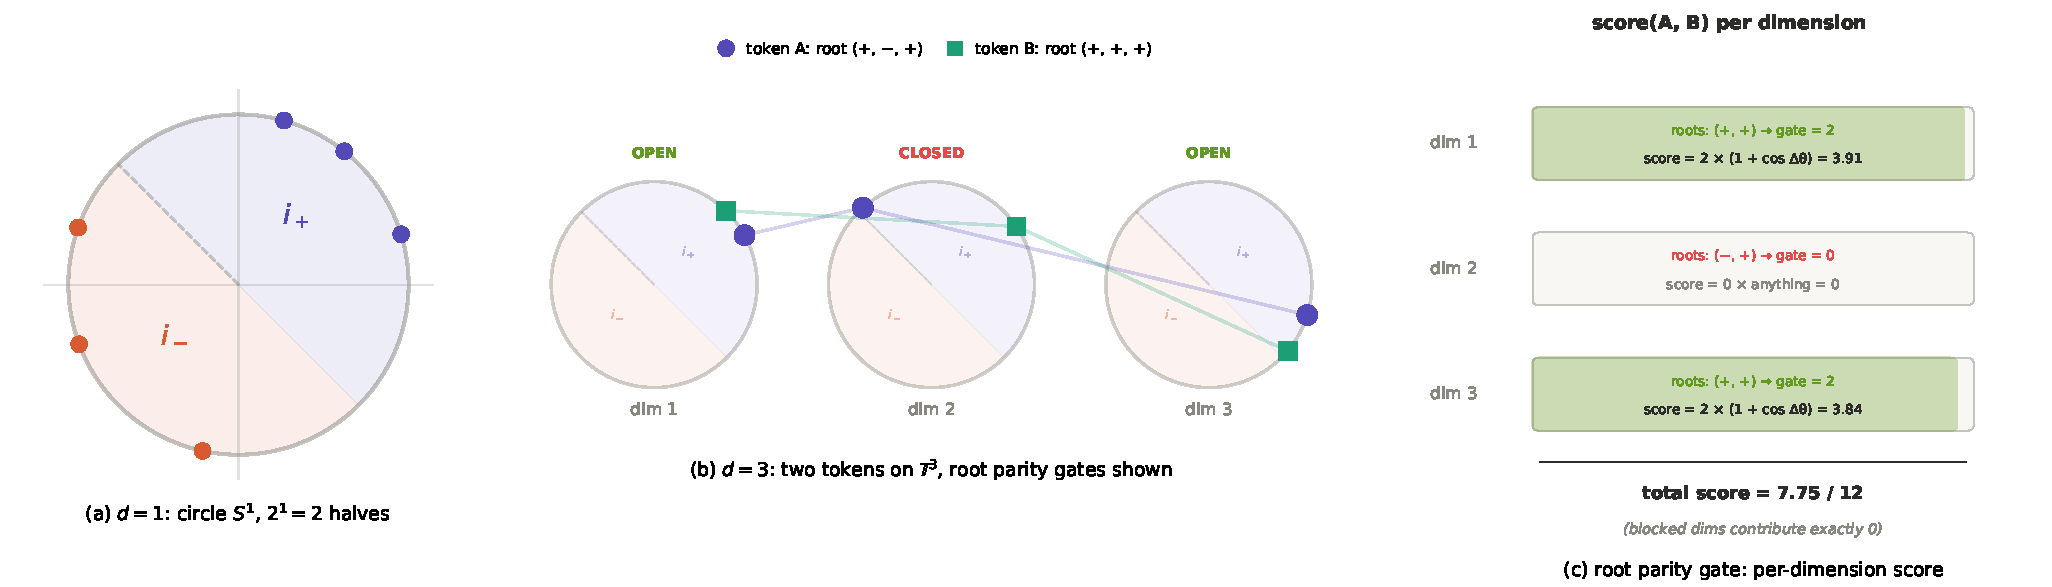
\includegraphics[width=\textwidth]{fig_torus.pdf}}{\fbox{\parbox{0.9\textwidth}{\centering\vspace{3em} [Figure: root-partitioned circles; include \texttt{fig\_torus.pdf} from the submission package] \vspace{3em}}}}
\caption{Root-parity labels on the $d$-torus. (a) A single circle $S^1$ divided into $i_+$ (purple) and $i_-$ (orange) halves by the root choice; tokens sit at their phase angle $\theta$. (b) Two tokens on $\mathbb{T}^3$ visualized as three independent circles: token A has root pattern $(+,-,+)$ and token B has $(+,+,+)$. The parity gate is open where roots match (dims 1 and 3) and closed where they differ (dim 2). (c) The per-dimension score: matching roots give gate $=2$ and a content score $2(1+\cos\Delta\theta)$; mismatched roots give gate $=0$ in the hard-root idealization. Tokens with different patterns still interact through their matching dimensions.}
\label{fig:torus}
\end{figure}

\subsection{Learned Phase Anchors}

The naive construction fixes the decision boundary at $\theta = \pi/4$ in absolute terms, so the network cannot move the dividing line between roots. We restore this freedom with a learned phase anchor $\omega_{h,d}$, one per head and dimension, shifting the boundary:
\begin{equation}
\beta = \cos(\theta + \omega) - \sin(\theta + \omega), \qquad \text{crossover at } \theta = \pi/4 - \omega.
\end{equation}
With $\omega$ initialized to $\pi/4$, the boundary begins at $\theta = 0$, so initially the sign of an activation determines its root. As training proceeds, each head and dimension can learn its own boundary. (Empirically, Section~\ref{sec:experiments} finds that at the 184M/1B-token scale the learned anchor does not improve over this initialization; we keep it for completeness and report the ablation.)

\section{Method}
\label{sec:method}

\subsection{Phase Generation and Soft Root Choice}
\label{sec:phasegen}

We project the input $x \in \R^D$ to queries, keys, and values in the standard way:
\begin{equation}
q = \frac{xW_q}{\sqrt{d}}, \quad k = \frac{xW_k}{\sqrt{d}}, \quad v = xW_v.
\end{equation}
Since the torus requires phases in $(-\pi, \pi)$ but $q, k$ are unbounded, we compress them with the element-wise map $\varphi(u) = \pi u / (1 + |u|)$, producing $\theta_q = \varphi(q)$ and $\theta_k = \varphi(k)$. This map is monotone and continuously differentiable ($C^1$); it is not smooth in the strict sense, as higher derivatives are discontinuous at $u = 0$. Large activations cluster near $\pm\pi$ while small activations remain locally linear. The root choice must be differentiable for end-to-end training, and we obtain a soft binarization via a sharp $\tanh$ on the shifted orientation amplitude:
\begin{equation}
r = \tanh\!\big(\gamma \cdot (\cos(\theta + \omega) - \sin(\theta + \omega))\big) \in (-1, 1).
\end{equation}
We fix $\gamma = 10$; $\gamma$ could equally be made learnable per head and dimension. Because the root is soft, the parity gate of Section~\ref{sec:sixpath} lies in the open interval $(0, 2)$ rather than in $\{0, 2\}$: nominally closed gates leak. Section~\ref{sec:gating-measured} quantifies this on the trained model: $|r| > 0.99$ on $87.8\%$ of activations, and the mean gate value on mismatched dimensions is $0.057$ (versus $2$ when open), so the realized gating is near-binary with roughly $3\%$ leakage.

\subsection{Bounded Temporal Phase Rotation}
\label{sec:rotation}

Position enters by rotating each phase as a function of sequence position. For a token at position $t$,
\begin{equation}
\theta^{\text{rot}} = \theta + t \cdot \lambda, \qquad \lambda = \tanh(\lambda_{\text{raw}}) \cdot \lambda_{\max},
\end{equation}
with $\lambda$ a learned per-(head, dimension) frequency, $\lambda_{\text{raw}}$ initialized at zero and $\lambda_{\max} = 0.01$. The rotation changes a token's phase but not its feature norm, and its contribution to the score is purely relative:
\begin{equation}
\cos(\theta^{\text{rot}}_q - \theta^{\text{rot}}_k) = \cos\big((\theta_q - \theta_k) + (t - j) \cdot \lambda\big).
\end{equation}
\textbf{Implementation disclosure.} The models evaluated in this paper additionally use a learned absolute positional embedding added to the token embeddings, which the earlier version of this work incorrectly stated was absent. This embedding caps the trained context at 2048 positions and means position is \emph{not} carried by the rotation alone in the reported experiments; removing it is a prerequisite for the length-extrapolation and streaming-beyond-training-context claims that the rotation-only design would otherwise permit, and is part of the follow-up architecture (Section~\ref{sec:limitations}). The ablation in Section~\ref{sec:experiments} finds that, with the absolute embedding present, the learned rotation does not contribute at this scale.

\subsection{The Root-Parity Feature Map}
\label{sec:sixpath}

The score should factorize into a parity gate and an angular similarity. This factorization is realized exactly by a six-channel construction (proof in Appendix~\ref{app:derivation}):
\begin{equation}
\boxed{\Phi(x) = \big[\, 1,\ \cos\theta^{\text{rot}},\ \sin\theta^{\text{rot}},\ r,\ r\cos\theta^{\text{rot}},\ r\sin\theta^{\text{rot}} \,\big]^\top \in \R^{6d}.}
\end{equation}
Writing $d'$ for the dimension index and $\Phi(q)_{d'}, \Phi(k)_{d'} \in \R^6$ for the per-dimension blocks,
\begin{equation}
\Phi(q)_{d'}^\top \Phi(k)_{d'} = \underbrace{(1 + r_{q,d'} \cdot r_{k,d'})}_{\text{root parity gate}} \cdot \underbrace{(1 + \cos(\theta^{\text{rot}}_{q,d'} - \theta^{\text{rot}}_{k,d'}))}_{\text{content + relative position}}.
\label{eq:parity}
\end{equation}

\begin{proposition}[Root Parity Gate, hard-root idealization]
For hard roots $r \in \{-1,+1\}$: when $r_{q,d'} = r_{k,d'}$, the gate equals $2$ and the per-dimension score ranges over $[0, 4]$; when $r_{q,d'} \neq r_{k,d'}$, the gate equals $0$ and the score is exactly zero regardless of content similarity.
\end{proposition}

With the soft $\tanh$ root used in practice, the factorization remains algebraically exact but the gate lies in $(0,2)$; the exact-zero property is an idealization whose realized approximation is measured in Section~\ref{sec:gating-measured}. A query thus draws primarily from tokens sharing its root label on each dimension, with cross-label contributions attenuated to the measured leakage level rather than eliminated.

\paragraph{A relaxed variant.} We also study a four-channel relaxation,
\[
\Phi_4(x) = [1,\; r,\; r\cos\theta^{\text{rot}},\; r\sin\theta^{\text{rot}}] \in \R^{4d},
\]
whose per-dimension score is $1 + r_q r_k(1 + \cos\Delta\theta)$: for matched hard roots $2 + \cos\Delta\theta \in [1,3]$, for mismatched $-\cos\Delta\theta \in [-1,1]$, so mismatch is no longer suppressed toward zero and gradient signal flows through blocked dimensions, at a $33\%$ smaller state ($4d \times d$). The earlier version of this work reported that this relaxation outperformed the strict gate; under the corrected evaluation protocol that finding is \emph{retracted}: the strict six-path gate outperforms the four-path relaxation in every configuration tested (Section~\ref{sec:experiments}).

\subsection{Power-Law Score Sharpening}
\label{sec:power}

Root parity makes the per-dimension score (near-)zero on mismatch; the activation must preserve this zero, which $\exp(\cdot)$ does not ($\exp(0)=1$ gives every blocked dimension a baseline contribution), while any positive power does. Let $s_{t,j} = \sum_{d'} \Phi(q_t)_{d'}^\top \Phi(k_j)_{d'} \in [0, 4d]$ be the raw score; we normalize and raise to a power:
\begin{equation}
\label{eq:powerlaw}
\text{attn}_{t,j} = \frac{\big(\tfrac{s_{t,j}}{4d}\big)^p}{\sum_{j' \leq t} \big(\tfrac{s_{t,j'}}{4d}\big)^p + \epsilon},
\end{equation}
with a causal mask applied before normalization and $\max(s,0)$ applied before exponentiation for the four-path variant (whose mismatch scores can be negative). We evaluate $p \in \{1, 2, 4\}$; only $p=1$ admits the exact recurrence below.

\subsection{Exact Constant-State Recurrence ($p=1$) and the Train--Inference Gap}
\label{sec:recurrent}

Training computes the full attention matrix in parallel; constant-memory decoding is the goal. At $p=1$ the factorized score permits exchanging the order of summation, turning per-step attention into two state updates:
\begin{equation}
S_t = S_{t-1} + \Phi(k_t)\, v_t^\top \in \R^{6d \times d}, \qquad z_t = z_{t-1} + \Phi(k_t) \in \R^{6d},
\end{equation}
with retrieval $\text{out}_t = \Phi(q_t)^\top S_t \,/\, (\Phi(q_t)^\top z_t + \epsilon)$. Each step costs $\cO(d^2)$ with a constant state of $6d^2 + 6d$ floats per head (96\,KB at $d=64$; 14.4\,MB for the full 12-layer, 12-head model in float32).

\paragraph{Verified exactness.} We implemented this recurrence and verified it against the parallel computation. On random weights, parallel and recurrent logits agree to $\sim 3\times 10^{-7}$ in float32. On the trained 184M $p=1$ model, held-out loss computed by the recurrence agrees with the parallel computation to within $10^{-4}$ nats (float32 accumulation with highest-precision matrix multiplication). Under reduced-precision TF32 matrix multiplication, pointwise logit deviations grow by roughly an order of magnitude, consistent with the float32 requirement for the phase pipeline stated in Section~\ref{sec:limitations}.

\paragraph{The $p>1$ train--inference gap, measured.} For $p > 1$, exact recurrence would require the $p$-th tensor power of $\Phi$, with state $\cO(d^{p+1})$. The earlier version of this work proposed treating the $p=1$ recurrence as an approximation for $p>1$-trained models; we measured this and \emph{withdraw that proposal}: the $p=2$ model degrades from 3.966 (parallel) to approximately 9.0 in held-out loss under the exact $p=1$ recurrence, and the $p=4$ model behaves similarly ($+3.5$ nats under an earlier protocol). The constant-state claim therefore holds only for models trained, or adapted, at $p=1$. The evaluated $p \in \{2,4\}$ models are fixed-context parallel attention variants, and are labeled as such throughout.

\paragraph{Two-stage recipe.} Single-stage $p=1$ training from scratch converges substantially more slowly than $p=2$ training under the same recipe and did not reach competitive loss within our budget. We therefore adopt a two-stage recipe: pretrain with the sharpened kernel ($p=2$), then adapt briefly at $p=1$ with a reduced learning rate. Adapting the 10B-token $p=2$ checkpoint for 0.63B tokens at learning rate $6\times10^{-5}$ yields a $p=1$ model at 3.951 held-out loss, statistically indistinguishable from its parallel $p=2$ parent (3.966), deployable with the exact constant state. (Adaptation at the pretraining rate $6\times10^{-4}$ destabilized the model; the reduced rate is part of the recipe.)

\section{Analysis}
\label{sec:analysis}

\subsection{The Address Space, Correctly Scoped}

\begin{theorem}[Per-Dimension Gating and Label Space]
\label{thm:address}
The six-path feature map (Eq.~\ref{eq:parity}) assigns each token a root label in $\{-1,+1\}^d$ and gates each dimension's contribution to the pairwise score by the agreement of the corresponding label bits. The $2^d$ count is the size of the label space. The full feature state occupies $6d^2 + 6d$ floats per head, independent of sequence length.
\end{theorem}

This statement is deliberately narrower than the ``$2^d$ interference-free sectors'' claim of the earlier version of this work, which was incorrect as stated: because the score \emph{sums} per-dimension gates, two tokens with different root patterns interact through every dimension on which their patterns agree, and with the soft root the gates are near-zero rather than zero on mismatch. What the mechanism provides is near-binary \emph{per-dimension} separation.

\subsection{Measured Gating Behavior}
\label{sec:gating-measured}

On the trained 10B-token model (layer 0, held-out inputs): $87.8\%$ of root activations satisfy $|r| > 0.99$, so the learned roots are near-binary in practice; the mean gate value on mismatched dimensions is $0.057$ (versus $2$ when open), i.e.\ leakage through nominally closed gates is approximately $3\%$; and token pairs mismatch on $49.3\%$ of dimensions on average, confirming that interaction through matching dimensions is the norm rather than the exception. Root parity is thus best understood as a strong, structured, per-dimension attenuation pattern, and its empirical value is isolated by ablation in Section~\ref{sec:experiments}: removing the root-gated channels entirely costs $+0.53$ nats at a matched budget.

\begin{proposition}
\label{prop:positivity}
For any query $q$ and accumulated state $z_t = \sum_{j \leq t}\Phi(k_j)$, $\Phi(q)^\top z_t \geq 0$ for hard roots, with strict positivity whenever some key matches the query's root on some dimension with non-antipodal phase.
\end{proposition}

The all-mismatch edge case is absorbed by the $\epsilon$ in Eq.~\ref{eq:powerlaw}, which therefore plays a genuine role.

\subsection{Inference Complexity, Correctly Accounted}

Per generated token with a KV cache, standard softmax attention costs $\cO(nd)$ compute and $\cO(nd)$ cache memory per head ($\cO(n^2 d)$ is the full-sequence training cost, not the per-step decode cost). The $p=1$ SANATAN recurrence costs $\cO(d^2)$ compute with $\cO(d^2)$ constant state. The evaluated $p \in \{2,4\}$ models decode as fixed-context parallel attention and carry no constant-state claim.

\subsection{Measured Memory/Latency Breakeven}
\label{sec:breakeven}

We benchmark the two decode mechanisms at the paper's configuration (12 layers, 12 heads, head dimension 64, float32) on a single workstation GPU, batch-1 decoding, mean over 50 steps after warmup. This is a mechanism-level microbenchmark isolating the attention decode path with matched unoptimized implementations of both mechanisms in the same framework.

\begin{center}
\small
\begin{tabular}{lccccc}
\toprule
Context $n$ & 1{,}024 & 2{,}048 & 8{,}192 & 32{,}768 & 131{,}072 \\
\midrule
Softmax KV cache (MB, all layers) & 75.5 & 151.0 & 604.0 & 2{,}415.9 & 9{,}663.7 \\
SANATAN state (MB, all layers) & \multicolumn{5}{c}{14.4 (constant; memory crossover at $n \approx 195$)} \\
\midrule
Softmax decode (ms/token) & 0.490 & 0.755 & 1.839 & 7.325 & --- \\
SANATAN recurrent step (ms/token) & \multicolumn{5}{c}{0.153 (constant in $n$)} \\
Speedup & $3.2\times$ & $4.9\times$ & $12.0\times$ & $47.9\times$ & --- \\
\bottomrule
\end{tabular}
\end{center}

The quality side of this trade is the $p=1$ result of Section~\ref{sec:experiments}: the constant-state model matches its parallel parent (3.951 versus 3.966). The trade is not free in training: SANATAN trains at $\approx$22K tokens/s on this hardware versus $\approx$78K for softmax and $\approx$121K for gated linear attention, due to trigonometric features, gating, and the expanded feature map; the memory and latency advantages are inference-time properties.

\section{Experiments}
\label{sec:experiments}

We evaluate SANATAN as a drop-in replacement for multi-head attention in a 184M-parameter causal language model (768 model dimension, 12 layers, 12 heads, head dimension 64, SwiGLU FFN 2048, RMSNorm pre-norm; LLaDA-8B-Instruct tokenizer, vocabulary 126{,}349, so 85.0M of 184M parameters are non-embedding). All models share the architecture, optimizer (AdamW, $\beta_1{=}0.9$, $\beta_2{=}0.95$, weight decay 0.1), learning rate $6\times10^{-4}$ with 500-step linear warmup, 2048-token context, and 65{,}536 tokens per step, differing only in the attention mechanism. Original SANATAN and kernel-baseline training ran on TPU v4-8; the corrected evaluations, the $p=1$ adaptation, the GLA baseline, and the decode benchmarks ran on a single workstation GPU.

\subsection{Corrected Evaluation Protocol}
\label{sec:protocol}

The earlier version of this work drew a separate small validation sample per training run from the \emph{head} of the streaming data mixture. This has two consequences we discovered during review: cross-run numbers are not comparable, and early checkpoints score anomalously well on the code-heavy head distribution, which produced the retracted result below. All numbers in this paper instead use a single common held-out set: 256 sequences of 2048 tokens, drawn with a fixed seed from \emph{deep} in each source stream (skipping 0.8M--4M documents per source, past all documents consumed by any training run), with token-level composition approximately 50\% FineWeb, 24\% StarCoder, 11\% CulturaX-zh, 8\% FineWeb-Edu, and 6\% math. All evaluations are float32.

We additionally disclose both mixture levels: the sampling weights (FineWeb 0.52, StarCoder 0.28, CulturaX-zh 0.11, FineWeb-Edu 0.06, OpenWebMath 0.015, FineMath 0.015) are \emph{document-draw} probabilities; because code documents are substantially longer, the realized token-level training mixture is approximately 85\% code.

\subsection{Main Results}

\begin{table}[t]
\centering
\caption{Held-out loss on the common protocol (lower is better; final checkpoints unless noted). All models: 184M-parameter class, identical tokenizer, data mixture, optimizer, and schedule. Token budgets differ and are stated. $p{>}1$ SANATAN rows are fixed-context parallel models; only the $p{=}1$ row carries the $\cO(d^2)$ constant-state property.}
\label{tab:results}
\small
\begin{tabular}{llccl}
\toprule
Model & Deployment form & Tokens & Held-out loss & Notes \\
\midrule
Gated Linear Attention~\cite{yang2024gla} & constant-state recurrent & 2.92B & \textbf{3.348} & matched recipe$^{a}$ \\
\midrule
SANATAN $p{=}1$ (two-stage) & \textbf{exact constant-state} & 10B $+$ 0.63B & 3.951 & recurrent $\equiv$ parallel$^{b}$ \\
SANATAN 6-path $p{=}2$ & fixed-context parallel & 10B & 3.966 & \\
SANATAN 6-path $p{=}4$ & fixed-context parallel & 1B & 5.377 & \\
\midrule
Linear Transformer~\cite{katharopoulos2020transformers} & constant-state recurrent & 3B & 4.524 & \\
Performer~\cite{choromanski2021rethinking} & constant-state recurrent & 3B & diverged & best ckpt 7.065 \\
Performer (stabilized) & constant-state recurrent & 3B & 8.767 & \\
cosFormer~\cite{qin2022cosformer} & constant-state recurrent & 3B & 9.806 & instability$^{c}$ \\
\midrule
Standard softmax & KV-cache & 3B & n/a & see Section~\ref{sec:softmax-note} \\
\bottomrule
\end{tabular}

\vspace{2pt}
{\footnotesize
$^{a}$flash-linear-attention implementation; 182.2M parameters with tied embeddings; best checkpoint at 2.92B of a 3B run; evaluated under bfloat16 autocast (all other rows float32). Training throughput on the same GPU: GLA $\approx$121K tokens/s, softmax $\approx$78K, SANATAN $\approx$22K.
$^{b}$Recurrent and parallel evaluation agree to within $10^{-4}$ nats (Section~\ref{sec:recurrent}).
$^{c}$Consistent with instability reports for shared recipes~\cite{qin2022cosformer}; we report best-ever and final values for all baselines in Appendix~\ref{app:changelog}.}
\end{table}

Three findings, in order of importance. \textbf{First}, the exact constant-state model retains the quality of its full parallel counterpart: 3.951 versus 3.966, with the recurrence verified numerically rather than assumed. This is, to our knowledge, the central property the mechanism was designed for, now measured. \textbf{Second}, SANATAN outperforms the converged value of every evaluated pre-2022 constant-memory attention baseline under the shared recipe (best: Linear Transformer at 4.524), with the caveat that the shared recipe destabilized several baselines (Performer diverged; cosFormer degraded), a recipe-sensitivity concern raised in review and confirmed by our own data; the claim is accordingly scoped to these baselines under this recipe. \textbf{Third}, and reported without qualification: a matched-recipe Gated Linear Attention baseline reaches 3.348 at 2.92B tokens, outperforming all SANATAN variants, including the $p=1$ model trained on substantially more tokens, while training $5.5\times$ faster. At this scale and recipe, SANATAN is not competitive with modern gated linear attention on language-modeling quality or training throughput. The contribution that survives this comparison is the mechanism and its verified constant-state form; whether root-parity gating can benefit stronger recurrent architectures is an open question (Section~\ref{sec:limitations}).

\subsubsection{On the Softmax Baseline}
\label{sec:softmax-note}

The earlier version of this work reported softmax at 3.27 versus SANATAN at 4.85; both numbers used the flawed per-run protocol and are not comparable to Table~\ref{tab:results}. The original softmax checkpoint was not retained. Two GPU retraining attempts under the shared recipe failed: the first due to a bfloat16 attention-precision issue absent on TPU (our SANATAN implementation computes attention internals in float32 explicitly and was unaffected; the softmax baseline implementation did not), and a full-precision retrain exhibited training instability. We therefore report no corrected softmax number rather than an unreliable one; the GLA baseline, which trains stably and strongly under the matched recipe, serves as the strong reference point. A stabilized softmax baseline on the common protocol remains future work.

\subsection{Ablations}

\begin{table}[t]
\centering
\caption{Ablations on the common held-out protocol (1B tokens each, final checkpoints, 6-path power$^2$ base unless stated). The earlier version of this work reported the 4-path variant as best (4.86); that result was an early-checkpoint artifact of the flawed protocol and is retracted (Appendix~\ref{app:changelog}).}
\label{tab:ablation}
\small
\begin{tabular}{lcc}
\toprule
Variant & Held-out loss & $\Delta$ \\
\midrule
6-path, power$^4$ & \textbf{5.377} & 0.00 \\
6-path, no learned $\omega$ (anchor fixed at init) & 5.393 & $+0.02$ \\
6-path, no temporal $\lambda$ & 5.477 & $+0.10$ \\
6-path, power$^2$ (full) & 5.578 & $+0.20$ \\
4-path, power$^4$ (relaxed gate) & 5.844 & $+0.47$ \\
4-path, power$^2$ (relaxed gate) & 5.965 & $+0.59$ \\
3-path (root-parity channels removed) & 6.110 & $+0.73$ \\
\bottomrule
\end{tabular}
\end{table}

The corrected ablation story differs from the earlier version in every particular worth noting. \textbf{Root parity carries real weight}: removing the three root-gated channels while keeping the angular kernel (3-path) costs $+0.53$ nats against the matched 6-path power$^2$ base (5.578 versus 6.110). \textbf{Sharpening helps}: power$^4$ improves on power$^2$ by $0.20$ nats. \textbf{The strict gate beats the relaxed gate everywhere}: 6-path outperforms 4-path at both exponents, reversing the retracted finding. \textbf{The learned anchor and the temporal rotation are not supported at this scale}: removing either matches or slightly improves the base, the latter plausibly because the absolute positional embedding (Section~\ref{sec:rotation}) already carries position. The useful diagnostic behind the retraction: checkpoints selected by the flawed head-of-stream validation score far worse on the common protocol (e.g., the Linear Transformer checkpoint that read 5.06 under the old protocol scores 6.616 on the common set, while its converged final checkpoint scores 4.524), confirming that the old protocol systematically favored early, code-overfit checkpoints.

\section{Related Work}
\label{sec:related}

\paragraph{Linear attention and modern recurrent models.} ELU-based linear attention~\cite{katharopoulos2020transformers} and Performer~\cite{choromanski2021rethinking} compress key--value pairs into $d \times d$ states with monotone or random feature maps; cosFormer~\cite{qin2022cosformer} adds cosine reweighting. RetNet~\cite{sun2023retnet}, RWKV~\cite{peng2023rwkv}, Mamba~\cite{gu2023mamba, gu2022efficiently}, and gated linear attention~\cite{yang2024gla} define the current competitive landscape for constant-memory sequence modeling, using learned decay or data-dependent gating of the recurrent state; GLA is our strongest evaluated baseline (Table~\ref{tab:results}). SANATAN differs in \emph{where} the gate acts: root parity gates the per-dimension query--key interaction via an algebraically derived binary label, rather than gating the state update. Whether these mechanisms compose is an open question we consider the most interesting raised by our results.

\paragraph{Rotation and polynomial activations.} Rotary position embedding~\cite{su2021roformer} encodes relative position by rotating queries and keys; relative positional encodings compatible with linear attention were developed by Liutkus et al.~\cite{liutkus2021spe} and unified and extended by Qin et al.~\cite{qin2023lrpe}, and ComRoPE~\cite{yu2025comrope} makes the rotation matrices trainable. SANATAN's temporal rotation is structurally related but operates inside the root-gated phase representation. Polynomial alternatives to softmax were studied by Saratchandran et al.~\cite{saratchandran2024rethinking} and, via sketching, by PolySketchFormer~\cite{kacham2023polysketchformer}; SANATAN's polynomial is constrained rather than incidental, since $(\cdot)^p$ preserves the (near-)zero gate that $\exp(\cdot)$ would erase.

\paragraph{Structured memory.} FlashAttention~\cite{dao2022flashattention} accelerates exact $\cO(n^2)$ attention; Linformer~\cite{wang2020linformer} projects to a fixed sequence size. Modern Hopfield networks~\cite{ramsauer2021hopfield} obtain exponential capacity through energy dynamics; SANATAN's label space is combinatorial, with capacity bounded by interference as discussed in Section~\ref{sec:analysis}. The algebraic starting point extends the author's prior work on the two matrix roots of $i^2=-1$ in complex-valued transformers~\cite{patel2025quantuminspired}; the contribution of the present paper is not the matrix-root observation but its use as a gated angular attention mechanism with a verified exact constant-state form. Distinguishing root-parity gating from learned binary gates, random or hash gates, and complex-valued attention via direct ablation remains future work.

\section{Conclusion, Limitations, and Future Work}
\label{sec:limitations}

SANATAN derives a per-dimension binary gate from the two matrix roots of $i^2 = -1$ and embeds it in an angular linear-attention kernel with an exact constant-state recurrent form. The corrected empirical record supports the following and no more: the recurrence is exact and verified ($\leq 10^{-4}$ nats agreement); a two-stage recipe preserves full parallel quality under the exact constant state (3.951 versus 3.966) where single-stage $p=1$ training and recurrent deployment of $p>1$ models (roughly $+5$ nats) do not; the constant state yields large measured decode advantages over softmax KV-caching ($3.2\times$--$48\times$ from 1K to 32K context at 14.4\,MB versus up to 2.4\,GB); root-parity gating contributes $+0.53$ nats over the ungated angular kernel; and SANATAN outperforms the evaluated pre-2022 constant-memory attention baselines under a shared recipe while remaining clearly behind matched-recipe gated linear attention (3.348) in both quality and training throughput.

\paragraph{Limitations.} Experiments are at a single scale (184M) and context (2048). The implementation's absolute positional embedding contradicts the rotation-only design and caps context; long-context and length-extrapolation evaluation (passkey retrieval, MQAR, downstream suites) requires the embedding-free variant and is not reported here. A corrected softmax baseline on the common protocol is unavailable (Section~\ref{sec:softmax-note}). The shared training recipe destabilized several baselines, so the kernel-baseline comparison bounds rather than settles their relative merits. Phase and root computations require float32. Each configuration was trained once. The gate sharpness $\gamma$ was fixed rather than learned. Training throughput is $3.5\times$ below softmax and $5.5\times$ below GLA on identical hardware.

\paragraph{Future work.} The follow-up architecture makes $\gamma$ learnable per head and dimension, removes the absolute positional embedding (making the recurrence valid at arbitrary position; verified exact at position offsets far beyond the trained context in preliminary implementation tests), and targets three questions in order: gate-construction ablations against learned, random, and hash gates; long-context evaluation under the exact recurrence; and, most importantly, whether root-parity interaction gating composes with the state-gating of modern architectures such as GLA, which our results identify as the stronger host.

\section*{Acknowledgments}
The author thanks the Google TPU Research Cloud (TRC) program for complimentary Cloud TPU access, and the NeurIPS 2026 reviewers and area chair of the earlier version, whose unusually precise reviews directly shaped the corrections, measurements, and scoping adopted here.

\bibliographystyle{unsrt}
\begin{thebibliography}{10}

\bibitem{vaswani2017attention}
A.~Vaswani, N.~Shazeer, N.~Parmar, J.~Uszkoreit, L.~Jones, A.~N.~Gomez, {\L}.~Kaiser, and I.~Polosukhin.
\newblock Attention is all you need.
\newblock In \emph{Advances in Neural Information Processing Systems (NeurIPS)}, volume~30, pages 5998--6008, 2017.

\bibitem{dao2022flashattention}
T.~Dao, D.~Y.~Fu, S.~Ermon, A.~Rudra, and C.~R\'{e}.
\newblock {FlashAttention}: Fast and memory-efficient exact attention with {IO}-awareness.
\newblock In \emph{Advances in Neural Information Processing Systems (NeurIPS)}, 2022.

\bibitem{wang2020linformer}
S.~Wang, B.~Z.~Li, M.~Khabsa, H.~Fang, and H.~Ma.
\newblock {Linformer}: Self-attention with linear complexity.
\newblock \emph{arXiv preprint arXiv:2006.04768}, 2020.

\bibitem{katharopoulos2020transformers}
A.~Katharopoulos, A.~Vyas, N.~Pappas, and F.~Fleuret.
\newblock Transformers are {RNNs}: Fast autoregressive transformers with linear attention.
\newblock In \emph{International Conference on Machine Learning (ICML)}, volume 119 of \emph{Proceedings of Machine Learning Research}, pages 5156--5165, 2020.

\bibitem{choromanski2021rethinking}
K.~Choromanski, V.~Likhosherstov, D.~Dohan, X.~Song, A.~Gane, T.~Sarlos, P.~Hawkins, J.~Davis, A.~Mohiuddin, L.~Kaiser, D.~Belanger, L.~Colwell, and A.~Weller.
\newblock Rethinking attention with {Performers}.
\newblock In \emph{International Conference on Learning Representations (ICLR)}, 2021.

\bibitem{sun2023retnet}
Y.~Sun, L.~Dong, S.~Huang, S.~Ma, Y.~Xia, J.~Xue, J.~Wang, and F.~Wei.
\newblock Retentive network: A successor to {Transformer} for large language models.
\newblock \emph{arXiv preprint arXiv:2307.08621}, 2023.

\bibitem{peng2023rwkv}
B.~Peng, E.~Alcaide, Q.~Anthony, A.~Albalak, S.~Arcadinho, S.~Biderman, H.~Cao, X.~Cheng, M.~Chung, M.~Grella, K.~K.~GV, X.~He, H.~Hou, J.~Lin, P.~Kazienko, J.~Kocon, J.~Kong, B.~Koptyra, H.~Lau, K.~S.~I.~Mantri, F.~Mom, A.~Saito, G.~Song, X.~Tang, B.~Wang, J.~S.~Wind, S.~Wozniak, R.~Zhang, Z.~Zhang, Q.~Zhao, P.~Zhou, Q.~Zhou, J.~Zhu, and R.-J.~Zhu.
\newblock {RWKV}: Reinventing {RNN}s for the {Transformer} era.
\newblock In \emph{Findings of the Association for Computational Linguistics: EMNLP}, 2023.

\bibitem{gu2023mamba}
A.~Gu and T.~Dao.
\newblock {Mamba}: Linear-time sequence modeling with selective state spaces.
\newblock \emph{arXiv preprint arXiv:2312.00752}, 2023.

\bibitem{yang2024gla}
S.~Yang, B.~Wang, Y.~Shen, R.~Panda, and Y.~Kim.
\newblock Gated linear attention transformers with hardware-efficient training.
\newblock In \emph{International Conference on Machine Learning (ICML)}, volume 235 of \emph{Proceedings of Machine Learning Research}, pages 56501--56523, 2024.

\bibitem{gu2022efficiently}
A.~Gu, K.~Goel, and C.~R\'{e}.
\newblock Efficiently modeling long sequences with structured state spaces.
\newblock In \emph{International Conference on Learning Representations (ICLR)}, 2022.

\bibitem{hoffmann2022training}
J.~Hoffmann, S.~Borgeaud, A.~Mensch, E.~Buchatskaya, T.~Cai, E.~Rutherford, D.~de~Las~Casas, L.~A.~Hendricks, J.~Welbl, A.~Clark, T.~Hennigan, E.~Noland, K.~Millican, G.~van~den~Driessche, B.~Damoc, A.~Guy, S.~Osindero, K.~Simonyan, E.~Elsen, J.~W.~Rae, O.~Vinyals, and L.~Sifre.
\newblock Training compute-optimal large language models.
\newblock In \emph{Advances in Neural Information Processing Systems (NeurIPS)}, 2022.

\bibitem{patel2025quantuminspired}
B.~Patel.
\newblock Quantum-inspired complex transformers: Resolving the fundamental algebraic ambiguity for enhanced neural representations.
\newblock In \emph{NeurIPS 2025 Workshop on Non-Euclidean Foundation Models and Geometric Learning}, 2025.
\newblock \url{https://openreview.net/forum?id=6R2H4KicNb}.

\bibitem{qin2022cosformer}
Z.~Qin, W.~Sun, H.~Deng, D.~Li, Y.~Wei, B.~Lv, J.~Yan, L.~Kong, and Y.~Zhong.
\newblock cos{F}ormer: Rethinking softmax in attention.
\newblock In \emph{International Conference on Learning Representations (ICLR)}, 2022.

\bibitem{ramsauer2021hopfield}
H.~Ramsauer, B.~Sch{\"a}fl, J.~Lehner, P.~Seidl, M.~Widrich, L.~Gruber, M.~Holzleitner, M.~Pavlovi{\'c}, G.~K.~Sandve, T.~Unterthiner, S.~Hochreiter, and G.~Klambauer.
\newblock Hopfield networks is all you need.
\newblock In \emph{International Conference on Learning Representations (ICLR)}, 2021.

\bibitem{su2021roformer}
J.~Su, Y.~Lu, S.~Pan, A.~Murtadha, B.~Wen, and Y.~Liu.
\newblock {RoFormer}: Enhanced transformer with rotary position embedding.
\newblock \emph{arXiv preprint arXiv:2104.09864}, 2021.

\bibitem{liutkus2021spe}
A.~Liutkus, O.~C{\'i}fka, S.-L.~Wu, U.~{\c{S}}im{\c{s}}ekli, Y.-H.~Yang, and G.~Richard.
\newblock Relative positional encoding for {Transformers} with linear complexity.
\newblock In \emph{International Conference on Machine Learning (ICML)}, volume 139 of \emph{Proceedings of Machine Learning Research}, pages 7067--7079, 2021.

\bibitem{qin2023lrpe}
Z.~Qin, W.~Sun, K.~Lu, H.~Deng, D.~Li, X.~Han, Y.~Dai, L.~Kong, and Y.~Zhong.
\newblock Linearized relative positional encoding.
\newblock \emph{Transactions on Machine Learning Research}, 2023.

\bibitem{yu2025comrope}
H.~Yu, T.~Jiang, S.~Jia, S.~Yan, S.~Liu, H.~Qian, G.~Li, S.~Dong, H.~Zhang, and C.~Yuan.
\newblock {ComRoPE}: Scalable and robust rotary position embedding parameterized by trainable commuting angle matrices.
\newblock In \emph{IEEE/CVF Conference on Computer Vision and Pattern Recognition (CVPR)}, pages 4508--4517, 2025.

\bibitem{saratchandran2024rethinking}
H.~Saratchandran, J.~Zheng, Y.~Ji, W.~Zhang, and S.~Lucey.
\newblock Rethinking attention: Polynomial alternatives to softmax in transformers.
\newblock \emph{arXiv preprint arXiv:2410.18613}, 2024.

\bibitem{kacham2023polysketchformer}
P.~Kacham, V.~Mirrokni, and P.~Zhong.
\newblock {PolySketchFormer}: Fast transformers via sketching polynomial kernels.
\newblock \emph{arXiv preprint arXiv:2310.01655}, 2023.

\end{thebibliography}

\appendix

\section{Derivation of the Root Parity Score Decomposition}
\label{app:derivation}

We prove that the six-path feature map $\Phi = [1, \cos\theta, \sin\theta, r, r\cos\theta, r\sin\theta]$ produces a per-dimension score that factors into a root parity gate and a content similarity term. The derivation is exact for any $r$; the gate takes values in $\{0,2\}$ for hard roots $r \in \{-1,+1\}$ and in $(0,2)$ for the soft $\tanh$ root used in training.

\paragraph{Setup.} For a single dimension $d'$, let $\theta_q, \theta_k$ denote the rotated phases of query and key, and $r_q, r_k$ their root values. The per-dimension feature blocks are
\begin{align}
\Phi(q)_{d'} &= (1,\; \cos\theta_q,\; \sin\theta_q,\; r_q,\; r_q\cos\theta_q,\; r_q\sin\theta_q), \\
\Phi(k)_{d'} &= (1,\; \cos\theta_k,\; \sin\theta_k,\; r_k,\; r_k\cos\theta_k,\; r_k\sin\theta_k).
\end{align}

\paragraph{Dot product expansion.} Using $\cos A \cos B + \sin A \sin B = \cos(A-B)$ twice,
\begin{align}
\Phi(q)_{d'}^\top \Phi(k)_{d'} &= 1 + \cos\Delta\theta + r_q r_k + r_q r_k \cos\Delta\theta \notag \\
&= (1 + r_q r_k)(1 + \cos\Delta\theta),
\end{align}
where $\Delta\theta = \theta_q - \theta_k$.

\paragraph{Root parity gate (hard roots).} When $r_q = r_k \in \{-1,+1\}$, $1 + r_q r_k = 2$; when $r_q \neq r_k$, $1 + r_q r_k = 0$:
\begin{equation}
\label{eq:rparity-cases}
\Phi(q)_{d'}^\top \Phi(k)_{d'} = \begin{cases} 2(1 + \cos\Delta\theta) \in [0, 4] & r_q = r_k, \\ 0 & r_q \neq r_k. \end{cases}
\end{equation}
This proves Proposition~1. With soft roots, $1 + r_q r_k \in (0, 2)$ and mismatch contributions are attenuated rather than zero; the realized attenuation is measured in Section~\ref{sec:gating-measured}.

\paragraph{Full score.} Summing over dimensions, $s_{t,j} = \sum_{d'} (1 + r_{q,d'} r_{k,d'})(1 + \cos\Delta\theta_{d'}) \in [0, 4d]$. For hard roots matching on $m$ of $d$ dimensions, $s \in [0, 4m]$; interaction between tokens with different patterns proceeds through their matching dimensions.

\paragraph{Denominator non-negativity (Proposition~\ref{prop:positivity}).} Each per-dimension term of $\Phi(q)^\top z_t = \sum_j \Phi(q)^\top \Phi(k_j)$ is a product of two non-negative factors ($1 + r_q r_k \geq 0$ and $1 + \cos\Delta\theta \geq 0$), hence non-negative; strict positivity holds whenever some key matches the query's root on some dimension with non-antipodal phase. The constant channel does not by itself provide a positive floor: the $r_q r_k$ term can equal $-1$ per dimension (hard roots), exactly canceling it, so the $\epsilon$ in Eq.~\ref{eq:powerlaw} genuinely handles the degenerate case.

\paragraph{Temporal rotation.} Substituting $\theta_q = \theta_{q,\text{content}} + t\lambda$ and $\theta_k = \theta_{k,\text{content}} + j\lambda$,
\begin{equation}
\Delta\theta = (\theta_{q,\text{content}} - \theta_{k,\text{content}}) + (t - j)\lambda,
\end{equation}
so content similarity and relative position enter the same cosine argument.

\section{Detailed Future Directions}
\label{app:future}

\paragraph{Spectral enrichment.} Replace the single cosine channel with harmonics $\{\cos(n\theta), \sin(n\theta)\}_{n \in \mathcal{N}}$ while retaining the root gate. For $\mathcal{N} = \{1, \ldots, N\}$ the per-dimension content score becomes $(1/N)\sum_{n=1}^{N}\cos(n\Delta\theta)$, a one-sided Dirichlet kernel that sharpens toward a delta at $\Delta\theta = 0$ as $N \to \infty$; the closed form evaluates at $\cO(1)$ cost in the parallel form, while the recurrent form requires $\cO(N)$ features per dimension.

\paragraph{Prime-frequency refinement.} Consecutive integer frequencies leave $O(1)$ secondary maxima at low-denominator rationals. Restricting $\mathcal{N}$ to distinct primes removes them: cyclic subgroups generated by distinct primes intersect only at the origin, so $\Delta\theta = 0$ is the unique common peak and off-peak values average to $O(1/\sqrt{K})$ for $K$ primes, a trigonometric analog of the Chinese Remainder Theorem.

\paragraph{Learnable angular resolution and gate sharpness.} A per-(head, dimension) frequency $\alpha = 1 + \tanh(\eta)$ replacing $\cos(\Delta\theta)$ with $\cos(\alpha\Delta\theta)$ provides learnable sharpness at no state cost, and the gate parameter $\gamma$ of Section~\ref{sec:phasegen} can likewise be made learnable (softplus-parameterized, initialized at the fixed value used here); both are implemented in the follow-up architecture.

\paragraph{Mechanism transfer.} The most consequential direction raised by Table~\ref{tab:results}: root parity gates the query--key \emph{interaction}, while GLA-family models gate the \emph{state update}; the two act on different parts of the recurrence and can in principle compose. Testing root-parity feature maps inside a GLA-style data-dependent-decay recurrence is the direct experiment.

\section{Changelog from the NeurIPS 2026 Submission}
\label{app:changelog}

For transparency, every substantive change from the reviewed version:

\begin{enumerate}
\item \textbf{Evaluation protocol replaced.} The submission's per-run head-of-stream validation sampling made cross-run numbers non-comparable and favored early checkpoints; all numbers now use the common seeded deep-stream held-out protocol of Section~\ref{sec:protocol}. For completeness, best-checkpoint versus final-checkpoint values on the common set: Linear Transformer 6.616/4.524 (the best checkpoint under the old protocol is an early, code-overfit one); Performer 7.065/diverged; Performer-stabilized 7.585/8.767; cosFormer 8.761/9.806; SANATAN 6-path $p{=}2$ 10B 3.969/3.966.
\item \textbf{Retraction: the four-path result.} The submission's headline ablation finding (4-path power$^4$ at 4.86, outperforming 6-path) was an artifact: that value came from a 0.09B-token checkpoint whose training subsequently degraded. On the common protocol the strict 6-path gate outperforms the 4-path relaxation in every configuration (Table~\ref{tab:ablation}).
\item \textbf{Constant-state claim restricted to $p{=}1$ and verified.} The submission reported $p \in \{2,4\}$ models with $\cO(d^2)$ inference and proposed the $p{=}1$ recurrence as an approximation for them; both are corrected. The recurrence is implemented and verified; the $p{>}1$ approximation is measured ($\approx{+}5$ nats) and withdrawn; the two-stage $p{=}1$ model (3.951) is the constant-state result.
\item \textbf{Complexity accounting corrected.} Softmax per-token decode is $\cO(nd)$ compute with $\cO(nd)$ KV memory, not $\cO(n^2 d)$ per step.
\item \textbf{Address-space claim narrowed.} ``$2^d$ interference-free sectors'' is replaced by per-dimension gating with the $2^d$ label-space interpretation, with measured gating statistics (Theorem~\ref{thm:address}, Section~\ref{sec:gating-measured}).
\item \textbf{Mathematical corrections.} $x^2=-1$ has two scalar solutions $\pm i$ (not a unique solution $i$); the non-orthogonal real $2\times2$ solution family has two degrees of freedom (not one); $S(\theta)$ is an orientation marker, not generally a root ($S(\theta)^2 = -(\cos\theta-\sin\theta)^2 I$); the soft gate lies in $(0,2)$, not $\{0,2\}$; $\varphi$ is $C^1$, not smooth.
\item \textbf{Positional-embedding disclosure.} The implementation uses a learned absolute positional embedding, contradicting the submission's ``without auxiliary positional embeddings'' claim (Section~\ref{sec:rotation}).
\item \textbf{Baselines.} Gated Linear Attention added under the matched recipe (3.348); the softmax comparison is withdrawn pending a stable retrain (Section~\ref{sec:softmax-note}); best-ever and final values reported for all baselines (item 1).
\item \textbf{New measurements.} Memory/latency breakeven (Section~\ref{sec:breakeven}); gating statistics (Section~\ref{sec:gating-measured}); recurrence equivalence and precision sensitivity (Section~\ref{sec:recurrent}); training throughput for all mechanisms.
\item \textbf{Framing.} ``Quantum-inspired'' and ``holographic'' removed from title and framing; both mixture levels disclosed (document-draw weights versus the $\approx 85\%$-code realized token mixture); Chinchilla-optimality framing dropped; three bibliography entries corrected (now \cite{liutkus2021spe, qin2023lrpe, yu2025comrope, saratchandran2024rethinking}) after an author-field error in each was identified during review.
\end{enumerate}

\end{document}
